\subsection{Model 1: known boundary, one $k$ per percept}

This model learns a set of waiting times, one per stimulus, so as to maximize overall reward rate (R-learning).
It should capture dependence of waiting time on stimulus difficulty and outcome \citep[Fig 3G]{lak2014orbitofrontal} and trial history \citep[Fig S3]{lak2014orbitofrontal}.

\subsubsection{Model description}

Stimulus is represented by $x \in X = \{5, 30, 45, 55, 70, 95 \}$, and the corresponding stimulus category $c \in \{0,1\} = H(x-50)$, where $H(z)$ is the Heaviside function
\begin{equation}
H(z) =
\begin{cases}
1 & \text{if }  z > 0 \\
0 & \text{if }  z < 0 \\
\end{cases}
\label{eq:heavi}
\nonumber
\end{equation}

The subject does not know the stimulus $x$, but the percept $\hat{x}$ defined as
\begin{equation}
    \hat{x} = \underset{x' \in X}{\operatorname{argmin}} \left( x' - x + \epsilon \right)
    \nonumber
\end{equation}
where $\epsilon$ is a Gaussian noise term.
That is to say, the\textbf{ percept is a noise corrupted stimulus rounded to the nearest element in the original stimulus set}.

On each trial, the subject makes two decisions:
\begin{enumerate}
    \item a perceptual decision $a = H(\hat{x} - 50)$ (ie. known boundary, no decision noise)
    \item a time investment (TI) decision $ k_{\hat{x}} \in \mathbb{R}_+ $
\end{enumerate}

A reward is earned whenever the perceptual choice $a$ is correct and waiting time ($k_{\hat{x}}$) is longer than reward delay $d$ ($d \sim Exp(1.5), d \in \left[0.5,8\right]$).

%\subsubsection{Learning $k_{\hat{x}}$}

The subject learns one TI value $k_{\hat{x}}$ per percept $\hat{x}$, and $k_{\hat{x}}$ is learned according to a delta learning rule that maximizes overall reward rate.

Reward rate $\rho$ is learned from experience as in \cite{constantino2015learning}.
For reward $r=1$ for rewarded trials and $0$ otherwise, and trial duration $\tau$, the learning target $\delta$ is defined as follows:
\begin{align}
\tau &=
\begin{cases}
d & \text{if trial rewarded} \\
k_{\hat{x}} & \text{if not rewarded}\\
\end{cases}\\
\delta &= r - \tau \rho
\nonumber
\end{align}

The actual updating equations are
\begin{align}
    k_{\hat{x}} &\leftarrow k_{\hat{x}} + \eta_k \delta \\
    \rho &\leftarrow \rho + (1-(1-\eta_\rho)^\tau) \delta
\end{align}
where $\eta_k, \eta_\rho \in [0,1]$ are learning rate parameters.

\subsubsection{Simulation}

This model captures several aspects of \cite{lak2014orbitofrontal}.
The psychometric looks reasonable, and waiting time depends on stimulus difficulty and whether choice was correct or incorrect (figure \ref{fig:mod1f3}).
As in figure S3 of \cite{lak2014orbitofrontal}, performance is the same irrespective of whether previous trial was correct or incorrect, or whether waiting time on previous trial was above or below median (long vs short) (figure \ref{fig:mod1fs3}).
Furthermore, waiting time is higher when previous trial was a long one.

Points where this model fails:
\begin{itemize}
    \item Waiting time does not depend on outcome of previous trial (figure \ref{fig:mod1fs3}, top right). \textbf{Fix}: make waiting time $k$ a function of reward probability (model 2); learn reward probability from experience (models 3-4); learn decision boundary.
    \item Target reward rate is not a fixed point; degrades after initial improvement (fig \ref{fig:mod1f3}, bottom right). \textbf{Fix}: Delta learning rule is intuitively ok, but defective; use a principled one (see below).
\end{itemize}

\begin{figure}[t!]
    \centering
    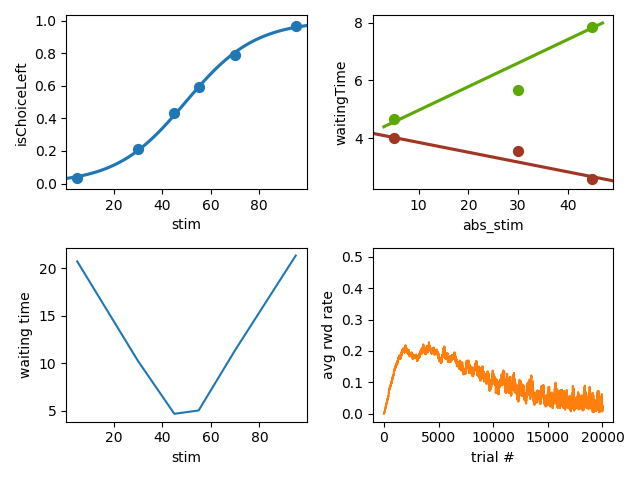
\includegraphics[width=.6\linewidth]{dual2afc/myplot.png}
    \caption{Model 1.\\
    (\textbf{top left}) Psychometric curve. \\
    (\textbf{top right}) Waiting time dependence on stimulus difficulty and outcome (green: correct, red: incorrect). \\
    (\textbf{bottom left}) Final values of $ k_\hat{x} $. \\
    (\textbf{bottom right}) Evolution of average reward rate $\rho$ through learning.}
    \label{fig:mod1f3}
\end{figure}

\begin{figure}[h!]
    \centering
    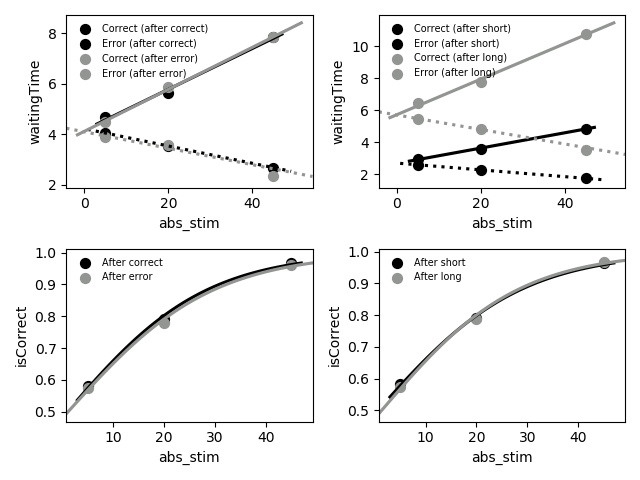
\includegraphics[width=.6\linewidth]{dual2afc/myplot2.png}
    \caption{Model 1. Plots analogous to figure S3 in \cite{lak2014orbitofrontal}}
    \label{fig:mod1fs3}
\end{figure}